In geometric optics, the so called eiconal equation
\begin{equation}
\biggl( \frac{\partial u}{\partial x}\biggr)^2
+
\biggl( \frac{\partial u}{\partial y}\biggr)^2
=
n(x,y)^2
\label{40000007:eikonal}
\end{equation}
plays an important role.
The solution $u(x,y)$ describes the propagation of a wave in an optical
medium with optical density $n(x,y)$.
The level curves of $u(x,y)$ are curves of equal phase of wave fronts.
In particular, the gradient of $u$ is always orthogonal to the wave front,
it follows the direction of travel of the wave.
\begin{teilaufgaben}
\item
Solve the equation
\eqref{40000007:eikonal}
using a separation ansatz of the form $u(x,y)=X(x) + Y(y)$ for 
\[
n(x,y)=
\begin{cases}n_1&\qquad x< 0\\
n_2&\qquad x>0.
\end{cases}
\]
\item
Compute the angles
$\alpha_1$ and $\alpha_2$
between the gradients of your solution and the $x$-axis for $x<0$ and
$x>0$.
Find 
$\sin\alpha_1/\sin\alpha_2$.
\end{teilaufgaben}

\begin{loesung}
\begin{figure}
\centering
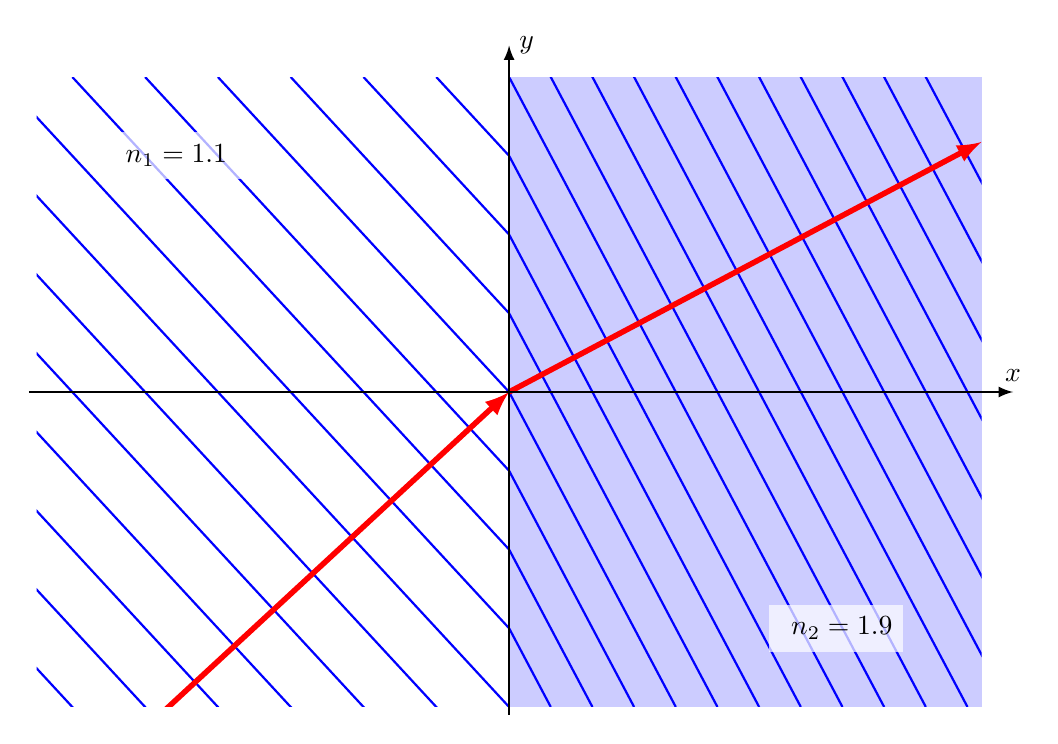
\begin{tikzpicture}[>=latex,thick]
\def\none{1.1}
\def\ntwo{1.9}
\def\l{0.2}
\fill[color=blue!20] (0,-4) rectangle (6,4);
\begin{scope}
\clip (-6,-4) rectangle (6,4);
\pgfmathparse{sqrt(\ntwo*\ntwo-\l*\l}
\xdef\m{\pgfmathresult}
\foreach \b in {-4,...,14}{
	\draw[color=blue] (0,\b) -- ({(\b+4)/\m},-4);
}
\draw[->,color=red,line width=2.0pt] (0,0)--(6,{6/\m});
\pgfmathparse{sqrt(\none*\none-\l*\l}
\xdef\m{\pgfmathresult}
\foreach \b in {-10,...,4}{
	\draw[color=blue] (0,\b) -- ({(\b-4)/\m},4);
}
\draw[->,color=red,line width=2.0pt] (-10,{-10/\m}) -- (0,0);
\end{scope}
\draw[->] (-6.1,0) -- (6.4,0) coordinate[label={$x$}];
\draw[->] (0,-4.1) -- (0,4.4) coordinate[label={right:$y$}];
\fill[color=white,opacity=0.7] (-5,2.7) rectangle (-3.3,3.3);
\node at (-5,3) [right] {$n_1=\none$\strut};
\fill[color=white,opacity=0.7] (3.3,-3.3) rectangle (5,-2.7);
\node at (5,-3) [left] {$n_2=\ntwo$\strut};
\end{tikzpicture}
\caption{Level curves (blue) of one of the the solutions of the
differential equation~\eqref{40000007:eikonal} for the particular
value $\lambda=1$ of the separation constant are straight lines with
slope $m=\sqrt{n_i^2-\lambda^2}/\lambda$.
The gradients are vectors perpendicular the level curves and are
shown in red.
They describe light rays through the medium.
The solution shows that Snell's law of refraction can be derived from
the eiconal equation.
\label{40000007:level}}
\end{figure}
In this case $n$ does not depend on $y$, so it is just a function
of the form $n(x,y)=n(x)$ of $x$ alone.
\begin{teilaufgaben}
\item
We use the separation ansatz
\[
u(x,y)=X(x) + Y(y).
\]
Substituting into the partial differential equation
\eqref{40000007:eikonal} gives the separated form
\[
n(x)^2-X'(x)^2=Y'(y)^2.
\]
The left hand side only depends on $x$, the right hand side only depends
on $y$, so both sides must be constant.
We call the common constant, which obviously must be positive, 
$\lambda^2$.
For 
$Y(y)$
we find the ordinary differential equation
\[
Y'(y)=\lambda \qquad\Rightarrow\qquad Y(y)=\lambda y+ C_y.
\]
On the other, the equation for $X(x)$ is
\[
X'(x)=\sqrt{n(x)^2-\lambda^2}.
\]
No we have to distinguish the cases $x<0$ and $x>0$.
In each case $n(x)$ is constant, so we have
\[
X'(x)=\sqrt{n_i^2-\lambda^2}
\qquad
\Rightarrow
\qquad
X(x)=x\sqrt{n_i^2-\lambda^2} + C_x.
\]
Thus the solution is
\[
u(x,y)=\lambda y + x\sqrt{n_i^2-\lambda^2} + C,
\]
where we have to take the value $n_1$ for $n_i$ in the case $x<0$
and $n_2$ in the case $x>0$.
We have collected the constants
$C_x$ and $C_y$ in a single new constant\footnote{This constant
is not important for the next steps or for the applications.
In applications, $u$ is the phase of the wave, an additive constant
is just a physically unimportant global phase shift.
In the next step we want to study the gradient of $u$, which is not
affected by the constant $C$.}
$C$.
Figure~\ref{40000007:level} shows the level lines of a solution in blue.
\item
The gradient is
\[
\operatorname{grad}u(x,y)
=
\begin{pmatrix}
\sqrt{n_i^2-\lambda^2}\\
\lambda
\end{pmatrix}.
\]
For the angle between $x$-axis and gradient we find
\[
\tan\alpha_i
=
\frac{\lambda}{\sqrt{n_i^2-\lambda^2}}
=
\frac1{\sqrt{\frac{n_i^2}{\lambda^2}-1}}.
\]
This is equivalent to
\[
\sin\alpha_i=\frac{\lambda}{n_i}.
\]
We conclude that
\[
\frac{ \sin\alpha_1}{\sin\alpha_2}=\frac{n_2}{n_1},
\]
this is Snell's law.
Figure~\ref{40000007:level} shows the gradients of the solutions
as red arrows.
\qedhere
\end{teilaufgaben}
\end{loesung}

\begin{diskussion}
The solution of the eiconal equation is the phase of a wave of the
form
$A(x,y)e^{iu(x,y)}$ in an approximation for very short wave lengths.
The eiconal equation can be derived from the electromagnetic field
equations (Maxwell's equations).
In this approximation, diffraction effects are not visible and the
law of refraction (Snell's law) is valid exactly.
\end{diskussion}
